%%%%%%%%%%%%%%%%%%%%%%%%%%%%%%%%%%%%%%%%%%%%%%%%%%%%%%%%%%%%%%%%%%%%%%%%%%%%%%%
% A clean template for an academic CV. This is a short summary version.
%
% Uses tabularx to create two column entries (date and job/edu/citation).
% Defines commands to make adding entries simpler.
%
%%%%%%%%%%%%%%%%%%%%%%%%%%%%%%%%%%%%%%%%%%%%%%%%%%%%%%%%%%%%%%%%%%%%%%%%%%%%%%%

\documentclass[9pt,a4paper]{article}

% Insert image file
\usepackage[dvipdfmx]{graphicx}

% Useful aliases
\newcommand{\OU}{The University of Osaka}

% Identifying information
\newcommand{\Title}{Curriculum Vit\ae\ Summary}
\newcommand{\FirstName}{Naoki}
\newcommand{\LastName}{Chihara}
\newcommand{\MyName}{\FirstName\ \LastName}
\newcommand{\Me}{\smartunderline{\FirstName\ \LastName}}  % For citations
\newcommand{\Email}{naoki88[at]sanken.osaka-u.ac.jp}
\newcommand{\PersonalWebsite}{c-naoki.vercel.app}
\newcommand{\LabWebsite}{www.dm.sanken.osaka-u.ac.jp}
\newcommand{\ORCID}{0009-0005-7061-8214}
\newcommand{\GitHubProfile}{C-Naoki}
\newcommand{\Linkedin}{c-naoki}
\newcommand{\Gscholar}{pq2b3jQAAAAJ}
\newcommand{\Twitter}{c_naoki13}

% Names
\newcommand{\Prof}[1]{Prof.\! #1}
\newcommand{\YSakurai}{Yasushi Sakurai}
\newcommand{\YMatsubara}{Yasuko Matsubara}
\newcommand{\RFujiwara}{Ren Fujiwara}
\newcommand{\MOnizuka}{Makoto Onizuka}

% URLs
\newcommand{\YSakuraiURL}{https://www.dm.sanken.osaka-u.ac.jp/~yasushi/index-j.html}
\newcommand{\YMatsubaraURL}{https://www.dm.sanken.osaka-u.ac.jp/~yasuko/}
\newcommand{\MOnizukaURL}{http://www-bigdata.ist.osaka-u.ac.jp/professor/onizuka/onizuka_en.html}

% Load packages
%%%%%%%%%%%%%%%%%%%%%%%%%%%%%%%%%%%%%%%%%%%%%%%%%%%%%%%%%%%%%%%%%%%%%%%%%%%%%%%

% Full Unicode support for non-ASCII characters
\usepackage[utf8]{inputenc}
\usepackage[english]{babel}
\usepackage[TU]{fontenc}

% Set main fonts
\usepackage[sfdefault]{atkinson}
\usepackage[ttdefault]{sourcecodepro}
% \usepackage[sfdefault]{FiraSans}

% For Japanese characters
\usepackage{xeCJK}
\setCJKmainfont{Noto Sans CJK JP}  % for Linux
% \setCJKmainfont{Noto Sans JP}  % for MacOS

% Icon fonts
\usepackage{fontawesome5}
\usepackage{academicons}
\newcommand{\faDblp}{\hspace{-0.20em}\raisebox{-0.25em}{
\includegraphics[height=1.1em]{./fig/dblp.png}}\hspace{-0.1em}}

% Disable hyphenation
\usepackage[none]{hyphenat}

% Control the font size
\usepackage{anyfontsize}

% For fancy and multipage tables
\usepackage{tabularx}
\usepackage{ltablex}

% For new environments
\usepackage{environ}

% Manage dates and times
\usepackage{datetime}

% Set the page margins
\usepackage{geometry}

% To get the total page numbers (\pageref{LastPage})
\usepackage{zref-totpages}

% Control spacing in enumerates
\usepackage{enumitem}

% Use custom colors
\usepackage[usenames,dvipsnames]{xcolor}

% Configure section titles
\usepackage{titlesec}

% Fancy header configuration
\usepackage{fancyhdr}

% Control PDF metadata and links
\usepackage[colorlinks=true]{hyperref}

% Underline
\usepackage{culine}
\usepackage[normalem]{ulem}
\usepackage{soul}

\usepackage{tikz}
\usepackage{fontspec} % if using lualatex or xelatex
\usetikzlibrary{calc}
\usepackage{expl3}

\newcommand{\smartunderline}[1]{%
  \tikz[baseline=(X.base)]{
    \node[inner sep=0pt, outer sep=0pt] (X) {\strut #1};
    \draw[line width=0.5pt]
      ([yshift=0.6ex]X.south west) -- ([yshift=0.6ex]X.south east);
  }%
}

% Add semi-bold
\DeclareRobustCommand{\sbseries}{\fontseries{sb}\selectfont}
\DeclareTextFontCommand{\textsb}{\sbseries}

% Template configuration
%%%%%%%%%%%%%%%%%%%%%%%%%%%%%%%%%%%%%%%%%%%%%%%%%%%%%%%%%%%%%%%%%%%%%%%%%%%%%%%

\geometry{%
  margin=12.5mm,
  headsep=0mm,
  headheight=0mm,
  footskip=5mm,
  includehead=true,
  includefoot=true
}

% Custom colors
\definecolor{mediumgray}{gray}{0.5}
\definecolor{lightgray}{gray}{0.9}
\definecolor{mediumblue}{HTML}{2060c2}
\definecolor{lightblue}{HTML}{a0c3ff}
\definecolor{mediumred}{HTML}{ca8a03}

% No indentation
\setlength\parindent{0cm}

% Increase the line spacing
\renewcommand{\baselinestretch}{1.1}
% and the spacing between rows in tables
\renewcommand{\arraystretch}{1.25}

% Remove space between items in itemize and enumerate
\setlist{nosep}

% Set the spacing and format of sections
\titleformat{\section}
  % {\normalfont\Large\mdseries} % format
  {\fontsize{16}{19}\mdseries}
  {} % label
  {0pt} % separation (left separation for hang)
  {} % text before title
  [\titlerule] % text after title
\titlespacing*{\section}
  {0pt} % left pad
  {0.1cm} % before
  {0cm} % after

% Disable number of sections. Use this instead of "section*" so that the sections still
% appear as PDF bookmarks. Otherwise, would have to add the table of contents entries
% manually.
\makeatletter
\renewcommand{\@seccntformat}[1]{}
\makeatother

% Define a new environment to place all CV entries in a 2-column table.
% Left column are the dates, right column the entries.
\newcommand{\TablePad}{\vspace{-0.2cm}}
\NewEnviron{EntriesTableDuration}{
\TablePad
\begin{tabularx}{\textwidth}{@{}p{0.10\textwidth}@{\hspace{0.02\textwidth}}p{0.88\textwidth}@{}}
  \BODY
\end{tabularx}
\TablePad
}
\NewEnviron{EntriesTableYear}{
\TablePad
\begin{tabularx}{\textwidth}{@{}p{0.05\textwidth}@{\hspace{0.01\textwidth}}p{0.94\textwidth}@{}}
  \BODY
\end{tabularx}
\TablePad
}
\NewEnviron{EntriesTablePublications}{
\TablePad
\begin{tabularx}{\textwidth}{@{}p{0.035\textwidth}@{\hspace{0.01\textwidth}}p{0.955\textwidth}@{}}
  \BODY
\end{tabularx}
\TablePad
}
\NewEnviron{EntriesTableRight}{
\TablePad
\begin{tabularx}{\textwidth}{@{}p{0.82\textwidth}@{\hspace{0.01\textwidth}}>{\raggedleft\arraybackslash}p{0.17\textwidth}@{}}
  \BODY
\end{tabularx}
\TablePad
}

% Macros to set the year and duration on the left column
\newcommand{\Duration}[2]{\fontsize{10pt}{0}\selectfont \texttt{#1-#2}}
\newcommand{\DurationYear}[4]{\fontsize{10pt}{0}\selectfont \texttt{#1\!\!\@ #2 -- #3\!\!\@ #4}}
\newcommand{\Year}[1]{\fontsize{10pt}{0}\selectfont \texttt{#1}}
\newcommand{\Ongoing}{present}
\newcommand{\Future}{future}

% Macros to add entries to the table
\newcommand{\AwardEntry}[4]{%
  \!{\hypersetup{urlcolor=black} \href{#2}{#1}#4} & \hfill #3 \\
}

% Macros to add links and mark publications
\newcommand{\DOI}[1]{
\!\!\!\:\!\!
\faBook{}
{\fontsize{11.5pt}{0}\selectfont {\usefont{T1}{SourceSansPro-TLF}{m}{sc} doi:}} \href{https://doi.org/#1}{#1}}
\newcommand{\Website}[1]{\href{https://#1}{#1}}
\newcommand{\Preprint}[1]{Preprint: \href{https://doi.org/#1}{#1}}
\newcommand{\GitHub}[1]{\faGithub{}\, \href{https://github.com/#1}{#1}}
\newcommand{\Data}[1]{\faChartBar{} doi: \href{https://doi.org/#1}{#1}}
\newcommand{\URL}[1]{
\!\!\!\!\!\:
\faLink{}
{\fontsize{11.5pt}{0}\selectfont {\usefont{T1}{SourceSansPro-TLF}{m}{sc} url:}} \href{https://#1}{#1}}
\newcommand{\video}[1]{\raisebox{-0.06ex}{\faYoutube{}}\, \href{https://youtu.be/#1}{#1}}

% Define command to insert month name and year as date
\newdateformat{monthyear}{\monthname[\THEMONTH]\ \THEDAY, \THEYEAR}

% Configure a fancy footer
\newcommand{\Separator}{\hspace{3pt}|\hspace{3pt}}
\newcommand{\FooterFont}{\footnotesize\color{mediumgray}}
\pagestyle{fancy}
\fancyhf{}
\lfoot{%
  \FooterFont{}
  \MyName{}
  \Separator{}
  \Title{}
}
\rfoot{%
  \FooterFont{}
  Last updated: \monthyear\today{}
  \Separator{}
  Page \thepage{}\space of\space \ztotpages
}
\renewcommand{\headrulewidth}{0pt}
\renewcommand{\footrulewidth}{1pt}
\preto{\footrule}{\color{lightgray}}

% Metadata for the PDF output and control of hyperlinks
\hypersetup{
  colorlinks,
  allcolors=mediumblue,
  breaklinks=true,
  pdftitle={\Title{} - \MyName},
  pdfauthor={\MyName},
}

%%%%%%%%%%%%%%%%%%%%%%%%%%%%%%%%%%%%%%%%%%%%%%%%%%%%%%%%%%%%%%%%%%%%%%%%%%%%%%%
\begin{document}

% Header
\begin{minipage}[t]{0.5\textwidth}
  {\fontsize{20pt}{0}\selectfont\MyName}
  % {\fontsize{17pt}{0}\selectfont ~(千原~直己)}
\end{minipage}
\begin{minipage}[t]{0.5\textwidth}
  \begin{flushright}
    \Title{}
  \end{flushright}
\end{minipage}
\\[-0.1cm]
\textcolor{lightgray}{\rule{\textwidth}{3pt}}
\vspace{-1.0em}

% Summary
\begin{figure}[h]
    \begin{tabular}{cc}
    \begin{minipage}[h]{0.5\textwidth}
      \vspace{-1.2em}
        \begin{tabular}[t]{ll}
          \textbf{Address} & SANKEN, \OU \\[-0.35em]
          & Mihogaoka 8-1, Ibaraki, Osaka 567-0047, Japan \\[-0.35em]
          \textbf{Email} & \href{mailto:\Email}{\Email} \\[-0.35em]
          & (please replace [at] with @) \\[-0.35em]
          \textbf{University} & \Website{www.osaka-u.ac.jp} \\[-0.35em]
          \textbf{Laboratory} & \Website{\LabWebsite} \\[-0.35em]
          \textbf{Website} & \Website{\PersonalWebsite} \\[-0.35em]
          \textbf{Last Updated Date} & \monthyear\today{}
        \end{tabular}
    \end{minipage} &
    \hspace{5.0em}
    \begin{minipage}[h]{0.5\textwidth}
      \centering
      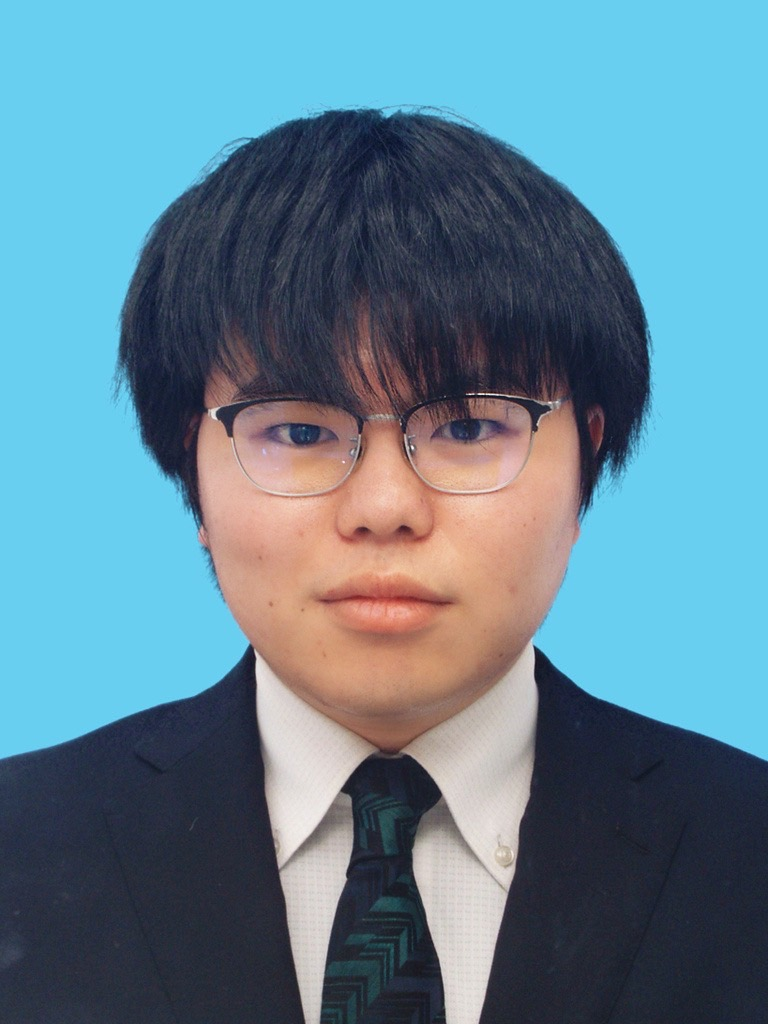
\includegraphics[width=0.3\linewidth]{./fig/profile.jpg}
    \end{minipage}
    \end{tabular}
\end{figure}
\vspace{-1.5em}

%%%%%%%%%%%%%%%%%%%%%%%%%%%%%%%%%%%%%%%%%%%%%%%%%%%%%%%%%%%%%%%%%%%%%%%%%%%%%%%
\section{About me}
\vspace{1.0em}
I am \MyName, a first-year Ph.D.\! student at \OU, Japan, and a specially appointed researcher at SANKEN (The Institute of Scientific and Industrial Research at \OU).
My research mainly focuses on data stream mining [C1, C2] and causal discovery in time series [C1].
I am fortunate to be advised by \href{\YSakuraiURL}{\Prof{\YSakurai}} and \href{\YMatsubaraURL}{\Prof{\YMatsubara}} at SANKEN.
I received my B.Sc.\! and M.Sc.\! degrees from \OU\ advised by \href{\MOnizukaURL}{\Prof{\MOnizuka}} and \href{\YSakuraiURL}{\Prof{\YSakurai}} in March 2023 and 2025, respectively.
\vspace{0.2em}
\\
\textbf{Keywords}:
\smartunderline{Time series analysis}, Data mining, \smartunderline{Stream processing}, \smartunderline{Causality}, Koopman operator theory, Missingness mechanisms, Time series forecasting, \smartunderline{Bayesian optimization}
\vspace{0.2em}
\\
\textbf{Links}:
~\faLinkedin{} \href{https://www.linkedin.com/in/\Linkedin}{Linkedin}
\Separator{}
\faGraduationCap{} \href{https://scholar.google.com/citations?hl=en&user=\Gscholar}{Google Scholar}
\Separator{}
\faGithub{} \href{https://github.com/\GitHubProfile}{GitHub}
\Separator{}
\faOrcid{} \href{https://orcid.org/\ORCID}{ORCID}
\Separator{}
\faTwitter{} \href{https://x.com/\Twitter}{Twitter}
\Separator{}
\faDblp{} \href{https://dblp.org/pid/363/1658.html}{DBLP}
\vspace{0.5em}

%%%%%%%%%%%%%%%%%%%%%%%%%%%%%%%%%%%%%%%%%%%%%%%%%%%%%%%%%%%%%%%%%%%%%%%%%%%%%%%
\section{Education}

\begin{EntriesTableRight}
  \textbf{Ph.D. in Information Science}, \OU
  \vspace{-0.1em}
  \newline
  \textcolor{gray}{{\fontsize{9pt}{0}\selectfont Department of Information Systems Engineering, Graduate School of Information Science and Technology}}
  \vspace{-0.1em}
  \newline
  {\setlength{\leftmargini}{17.2pt}
  \begin{itemize}
  \vspace{-1.0em}
      \item Exptected graduation date is March 2028
      \item Supervisor: \Prof{\YSakurai}
  \vspace{-1.3em}
  \end{itemize}}
  &
  \hfill
  \Duration{2025}{\Ongoing}
  \vspace{0.30em}
  \newline
  \hfill
  \textcolor{gray}{\fontsize{9pt}{0}\selectfont \texttt{Osaka, \!\!Japan}~}
  \\[4.45em]
  \textbf{M.Sc.\! in Information Science}, \OU
  \vspace{-0.1em}
  \newline
  \textcolor{gray}{{\fontsize{9pt}{0}\selectfont Department of Information Systems Engineering, Graduate School of Information Science and Technology}}
  \vspace{-0.1em}
  \newline
  {\setlength{\leftmargini}{17.2pt}
  \begin{itemize}
  \vspace{-1.0em}
      \item Thesis: Stream Mining Time-evolving Causality for Time Series Forecasting
      \item Supervisor: \Prof{\YSakurai}
  \vspace{-1.3em}
  \end{itemize}}
  &
  \hfill
  \Duration{2023}{2025}
  \vspace{0.5em}
  \newline
  \hfill
  \textcolor{gray}{\fontsize{9pt}{0}\selectfont \texttt{Osaka, \!\!Japan}~}
  \\[4.45em]
  \textbf{B.Sc.\! in Engineering}, \OU
  \vspace{-0.1em}
  \newline
  \textcolor{gray}{{\fontsize{9pt}{0}\selectfont Department of Electronic and Information Engineering, School of Engineering}}
  \vspace{-0.1em}
  \newline
  {\setlength{\leftmargini}{17.2pt}
  \begin{itemize}
  \vspace{-1.0em}
      \item Thesis: Detection of Variable Celestial Objects using Machine Learning-based Periodic Analysis and Domain Knowledge
      \item Supervisor: \Prof{\MOnizuka}
  \vspace{-1.3em}
  \end{itemize}}
  &
  \hfill
  \Duration{2019}{2023}
  \vspace{0.5em}
  \newline
  \hfill
  \textcolor{gray}{\fontsize{9pt}{0}\selectfont \texttt{Osaka, \!\!Japan}~}
\end{EntriesTableRight}

%%%%%%%%%%%%%%%%%%%%%%%%%%%%%%%%%%%%%%%%%%%%%%%%%%%%%%%%%%%%%%%%%%%%%%%%%%%%%%%
\section{Experience}

\begin{EntriesTableRight}
  \textbf{Japan Society for the Promotion of Science (JSPS)}
  \vspace{-0.1em}
  \newline
  \textcolor{gray}{\fontsize{9pt}{0}\selectfont Research Fellow DC1}
  &
  \hfill \Duration{2025}{\Ongoing}
  \vspace{0.25em}
  \newline
  \hfill \textcolor{gray}{\fontsize{9pt}{0}\selectfont \texttt{Osaka, \!\!Japan}~}
  \\
  \textbf{SANKEN}, \OU
  \vspace{-0.1em}
  \newline
  \textcolor{gray}{\fontsize{9pt}{0}\selectfont Specially Appointed Researcher}
  &
  \hfill \Duration{2023}{\Ongoing}
  \vspace{0.25em}
  \newline
  \hfill \textcolor{gray}{\fontsize{9pt}{0}\selectfont \texttt{Osaka, \!\!Japan}~}
  \\
  \textbf{School of Engineering}, \OU
  \vspace{-0.1em}
  \newline
  \textcolor{gray}{\fontsize{9pt}{0}\selectfont Teaching Assistant for ``Exercises in Mathematical Analysis''}
  &
  \hfill \Year{2023}
  \vspace{0.45em}
  \newline
  \hfill \textcolor{gray}{\fontsize{9pt}{0}\selectfont \texttt{Osaka, \!\!Japan}~}
  \\
  \textbf{Graduate School of Information Science and Technology}, \OU
  \vspace{-0.1em}
  \newline
  \textcolor{gray}{\fontsize{9pt}{0}\selectfont Assistant in the detection of variable celestial objects}
  &
  \hfill \Duration{2021}{2023}
  \vspace{0.45em}
  \newline
  \hfill \textcolor{gray}{\fontsize{9pt}{0}\selectfont \texttt{Osaka, \!\!Japan}~}
  \\
  \textbf{Nagase Co., Ltd.}
  \vspace{-0.1em}
  \newline
  \textcolor{gray}{\fontsize{9pt}{0}\selectfont Digital Technology Engineer}
  &
  \hfill \Duration{2020}{2023}
  \vspace{0.45em}
  \newline
  \hfill \textcolor{gray}{\fontsize{9pt}{0}\selectfont \texttt{Tokyo, \!\!Japan}~}
\end{EntriesTableRight}

% %%%%%%%%%%%%%%%%%%%%%%%%%%%%%%%%%%%%%%%%%%%%%%%%%%%%%%%%%%%%%%%%%%%%%%%%%%%%%%%
% \section{Community Service}

% \begin{EntriesTableDuration}
%   \Duration{2024}{\Ongoing} & \textbf{Embaixador}, Rede Brasileira de Reprodutibilidade, \Website{www.reprodutibilidade.org}
%   \\
%   \Duration{2024}{\Ongoing} & \textbf{Advisory Council Member}, EarthArXiv, \Website{eartharxiv.org}
%   \\
%   \Duration{2022}{\Ongoing} & \textbf{Board Member}, Software Underground, \Website{softwareunderground.org}
%   \\
%   \Duration{2022}{2023} & \textbf{Advisory Committee Member}, pyOpenSci, \Website{www.pyopensci.org}
%   \\
%   \Duration{2019}{2022} & \textbf{Topic Editor}, Journal of Open Source Software, \Website{joss.theoj.org}
% \end{EntriesTableDuration}

% %%%%%%%%%%%%%%%%%%%%%%%%%%%%%%%%%%%%%%%%%%%%%%%%%%%%%%%%%%%%%%%%%%%%%%%%%%%%%%%
% \section{Open Educational Resources}

% \begin{EntriesTableYear}
%   \Year{2022} &
%   \textbf{A Quick Introduction to Machine Learning}.
%   \GitHub{leouieda/ml-intro}.
%   \\
%   \Year{2023} &
%   \textbf{Remote Sensing with Python}.
%   \GitHub{leouieda/remote-sensing}.
%   \\
%   \Year{2023} &
%   \textbf{Lithosphere Dynamics with Python}.
%   \GitHub{leouieda/lithosphere}.
%   \\
%   \Year{2022} &
%   \textbf{Terrestrial Gravimetry with Python}.
%   \GitHub{leouieda/gravity-processing}.
% \end{EntriesTableYear}


%%%%%%%%%%%%%%%%%%%%%%%%%%%%%%%%%%%%%%%%%%%%%%%%%%%%%%%%%%%%%%%%%%%%%%%%%%%%%%%
\section{Grants and Awards}

\begin{EntriesTableRight}
  \AwardEntry{Award of the Graduate School of Information Science and Technology of Osaka University}{}{ \Year{Mar \!2025}}{}
  \AwardEntry{DEIM2025 Student Presentation Award}{}{ \Year{Mar \!2025}}{}
  \AwardEntry{\textbf{Information Processing Society of Japan (IPSJ) Yamashita SIG Research Award}}{https://www.ipsj.or.jp/award/yamasita2024-detail.html\#dbs}{\Year{Jul \!2024}}{}
  \AwardEntry{DEIM2024 Best Paper Award Runner-up}{https://confit.atlas.jp/guide/event/deim2024/static/awards}{\Year{Jun \!2024}}{ (top 1.4\%)}
  \AwardEntry{Osaka University Humanware Innovation Program Scholarship}{}{ \Duration{2023}{\Ongoing}}{}
\end{EntriesTableRight}

%%%%%%%%%%%%%%%%%%%%%%%%%%%%%%%%%%%%%%%%%%%%%%%%%%%%%%%%%%%%%%%%%%%%%%%%%%%%%%%
\section{Publications}

\vspace{1.0em}
{\fontsize{12pt}{0}\textbf{Peer-reviewed Publications}}
\begin{EntriesTablePublications}
  % [C3] &
  % \Me, \RFujiwara, \YMatsubara, and \YSakurai.
  % \textbf{Causal Discovery from Time Series under Missing Data Mechanisms}.
  % (Under submission to NeurIPS).
  % \\

  [C2] &
  \Me, \RFujiwara, \YMatsubara, and \YSakurai.
  \textbf{Nova: Learning Nonlinear Time-varying Dynamical Systems from Data Streams with Koopman Operator}.
  (Under submission to SIGKDD).
  \\

[C1] &
  \Me, \YMatsubara, \RFujiwara, and \YSakurai.
  \textbf{Modeling Time-evolving Causality over Data Streams}.
  Proceedings of the 31st ACM SIGKDD Conference on Knowledge Discovery and Data Mining (\textbf{KDD '25}), Toronto, ON, Canada, August 3-7, 2025. Acceptance rate: 19\%. \DOI{10.1145/3690624.3709283}.
  \newline
  \hspace*{-0.12em}
  \GitHub{C-Naoki/ModePlait}
  \Separator{}
  \video{01hS6R1a8jg}
  \\

[W1] &
  \Me, \YMatsubara, \RFujiwara, and \YSakurai.
  \textbf{Stream Mining Time-evolving Causality in Time Series}.
  The 30th ACM SIGKDD Conference on Knowledge Discovery and Data Mining (KDD '24) PhD Consortium, Barcelona, Spain, August 25-29, 2024.
  \URL{kdd2024.kdd.org/ph-d-consortium}.
  \\

[J2] &
  \Me, \YMatsubara, \RFujiwara, and \YSakurai.
  \textbf{Real-time Forecasting of Time-evolving Data Streams using Dynamic Mode Decomposition}.
  IPSJ Transactions on Databases (TOD), Vol. 17, No. 2, pp. 1-11, April 23, 2024. \URL{ipsj.ixsq.nii.ac.jp/records/233825}.
  \\

[J1] &
  \Me, Tadafumi Takata, Yasuhiro Fujiwara, Koki Noda, Keisuke Toyoda, Kaito Higuchi, and \MOnizuka.
  \textbf{Effective detection of variable celestial objects using machine learning-based periodic analysis}.
  Astronomy and Computing, Vol. 45, pp. 100765, November 3, 2023. \DOI{10.1016/j.ascom.2023.100765}.
  \\

\end{EntriesTablePublications}

{\fontsize{12pt}{0}\textbf{Non-refereed Publications}}

\begin{EntriesTablePublications}
[N4] &
  \Me, \YMatsubara, \RFujiwara, and \YSakurai.
  \textbf{時間変化する因果関係の抽出に基づいた高速将来予測}.
  The 17th Forum on Data Engineering and Information Management (DEIM2025), Fukuoka, Japan, February 27 - March 4, 2025.
  \newline
  \textcolor{mediumred}{\textsb{Student Presentation Award.}}
\\

[N3] &
  \Me, \YMatsubara, \RFujiwara, and \YSakurai.
  \textbf{動的モード分解を活用した高速将来予測アルゴリズム}.
  The 16th Forum on Data Engineering and Information Management (DEIM2024), Hyogo, Japan, February 28 - March 5, 2024.
  \newline
  \textcolor{mediumred}{\textsb{Best Paper Award Runner-up, IPSJ Yamashita SIG Research Award.}}
  \\

[N2] &
  Aiyi Li, Kenya Hoshimure, Kei Tanigaki, Yota Hatano, Reina Nozawa, Yuki Sakamoto, Yuanzhou Wei, \Me, and Naoki Kodani.
  \textbf{Semi-autonomous Leader-follower Approach for Swarm Drone Guidance}.
  The 36th SICE Symposium on Decentralized Autonomous Systems, Tokyo, Japan, February 16-17, 2024.
  \\

[N1] &
  \Me, Tadafumi Takata, Yasuhiro Fujiwara, and \MOnizuka.
  \textbf{周期解析による変動天体の検出}.
  The 15th Forum on Data Engineering and Information Management (DEIM2023), Gifu, Japan, March 5-9, 2023.
\end{EntriesTablePublications}

{\fontsize{12pt}{0}\textbf{Patents}}

\begin{EntriesTablePublications}
  [P1] & Yasuhiro Fujiwara, \MOnizuka, and \Me.
  \textbf{検出装置、検出⽅法及びプログラム}.
  特開2025-000129, January 7, 2025. \URL{jglobal.jst.go.jp/detail?JGLOBAL\_ID=202503009056531197}.
\end{EntriesTablePublications}

%%%%%%%%%%%%%%%%%%%%%%%%%%%%%%%%%%%%%%%%%%%%%%%%%%%%%%%%%%%%%%%%%%%%%%%%%%%%%%%
\section{Academic Services}

\vspace{1.0em}
{\fontsize{11pt}{0}\textbf{External Reviewers}}

\begin{tabular}{cc}
  \begin{minipage}[h]{0.17\textwidth}
    {\setlength{\leftmargini}{17.2pt}
    \begin{itemize}
      \vspace{0.9em}
      \item ACM WWW
      \item ACM SIGKDD
    \end{itemize}}
  \end{minipage} &
  \begin{minipage}[h]{0.83\textwidth}
    {\setlength{\leftmargini}{-5pt}
    \begin{itemize}
      \vspace{0.9em}
      \item[] 2025
      \item[] 2025
    \end{itemize}}
  \end{minipage}
\end{tabular}

\vspace{1.0em}
{\fontsize{11pt}{0}\textbf{Conference Volunteer Work}}

\begin{tabular}{cc}
  \begin{minipage}[h]{0.17\textwidth}
    {\setlength{\leftmargini}{17.2pt}
    \begin{itemize}
      \vspace{0.5em}
      \item PAKDD
      % \item[]
    \end{itemize}}
  \end{minipage} &
  \begin{minipage}[h]{0.83\textwidth}
    {\setlength{\leftmargini}{-5pt}
    \begin{itemize}
      \vspace{0.5em}
      \item[] 2023
      % \item[]
    \end{itemize}}
  \end{minipage}
\end{tabular}

\end{document}
